\chapter{Reference Manuals for the \why Tools}
\label{chap:manpages}

This chapter details the usage of each of the command-line tools
provided by the \why environment. These are as follows:
\begin{description}
\item[\texttt{why3config}] tool for managing the user's configuration,
  including the detection of installed provers.
\item[\texttt{why3}] reads \why\ and \whyml input files and calls
  provers, on the command-line.
\item[\texttt{why3ide}] graphical interface to display goals, run
  provers and transformations on them.
\item[\texttt{why3replayer}] replay the proofs stored in a session,
  for regression test purposes
\item[\texttt{why3bench}] produces benchmarks.
\item[\texttt{why3session}] dumps various informations from a proof
  session, and possibly modifies the session.
\item[\texttt{why3doc}] produces HTML versions of \why source codes.
\end{description}

All these tools accept a common subset of command-line options. In
particular the option \verb|-help| which displays the usage and options.
\begin{description}
\item[\texttt{-L} $d$]
  adds $d$ in the load path, to search for theories.
\item[\texttt{-{}-library} $d$]
  same as \verb|-L|
\item[\texttt{-I} $d$]
  same as \verb|-L| (deprecated)
\item[\texttt{-C} $file$]
  reads configuration from $file$
\item[\texttt{-{}-config} $file$]
  same as \verb|-C|
\item[\texttt{-{}-extra-config} $file$]
  reads additional configuration from $file$
\item[\texttt{-{}-list-debug-flags}]
  lists known debug flags
\item[\texttt{-{}-debug-all}]
  sets all debug flags (except flags which change the behavior)
\item[\texttt{-{}-debug} $flag$]
  set a debug flag
\item[\texttt{-v}]
  print version information
\item[\texttt{-help}]
  displays the usage and the exact list of options for the given tool
\end{description}

\section{The \texttt{why3config} command-line tool}
\label{sec:why3config}

\why must be configured to access external provers. Typically, this is done
by running
%%either
the command line tool \texttt{why3config}.
%%or using the menu
%%\begin{verbatim}
%%File/Detect provers
%%\end{verbatim}
%%of the IDE.
This must be redone each time a new prover is installed.

The provers which \why attempts to detect are described in
the readable configuration file \texttt{provers-detection-data.conf}
of the \why data directory (\eg{}
\texttt{/usr/local/share/why3}). Advanced users may try to modify this
file to add support for detection of other provers. (In that case,
please consider submitting a new prover configuration on the bug
tracking system).

The result of provers detection is stored in the user's
configuration file (\verb+~/.why3.conf+ or, in the case of local
installation, \verb+why3.conf+ in Why3 sources top directory). This file
is also human-readable, and advanced users may modify it in order to
experiment with different ways of calling provers, \eg{} different
versions of the same prover, or with different options.

\texttt{why3config} also detects the plugins installed in the \why
plugins directory (\eg{} \texttt{/usr/local/lib/why3/plugins}). A
plugin must register itself as a parser, a transformation or a
printer, as explained in the corresponding section.

If the user's configuration file is already present,
\texttt{why3config} will only reset unset variables to default value,
but will not try to detect provers.
The option \verb|--detect-provers| should be used to force
\why to detect again the available
provers and to replace them in the configuration file. The option
\verb|--detect-plugins| will do the same for plugins.

If a supported prover is installed under a name
that is not automatically recognized by \texttt{why3config},
the option \verb|--add-prover| will add a specified binary
to the configuration. For example, an Alt-Ergo executable
\verb|/home/me/bin/alt-ergo-trunc| can be added as follows:
\begin{verbatim}
why3config --add-prover alt-ergo /home/me/bin/alt-ergo-trunc
\end{verbatim}
As the first argument, one should put a prover
identification string. The list of known prover identifiers
can be obtained by the option \verb|--list-prover-ids|.

\section{The \texttt{why3} command-line tool}
\label{sec:why3ref}

\why is primarily used to call provers on goals contained in an
input file. By default, such a file must be written either in \why language
(extension \texttt{.why}) or in \whyml language (extension \texttt{.mlw}).
However, a dynamically loaded
plugin can register a parser for some other format of logical problems,
\eg{} TPTP or SMTlib.

The \texttt{why3} tool executes the following steps:
\begin{enumerate}
\item Parse the command line and report errors if needed.
\item Read the configuration file using the priority defined in
  Section~\ref{sec:whyconffile}.
\item Load the plugins mentioned in the configuration. It will not
  stop if some plugin fails to load.
\item Parse and typecheck the given files using the correct parser in order
  to obtain a set of \why theories for each file. It uses
  the filename extension or the \verb|--format| option to choose
  among the available parsers. The \verb|--list-format| option gives
  the list of registered parsers.
  \whyml modules are turned into
  theories containing verification conditions as goals.
\item Extract the selected goals inside each of the selected theories
  into tasks. The goals and theories are selected using the options
  \verb|-G/--goal| and \verb|-T/--theory|. The option
  \verb|-T/--theory| applies to the last file appearing on the
  command line, the option \verb|-G/--goal| applies to the last theory
  appearing on the command line. If no theories are selected in a file,
  then every theory is considered as selected. If no goals are selected
  in a theory, then every goal is considered as selected.
\item Apply the transformation requested
  with \verb|-a/--apply-transform| in their order of appearance on the
  command line. \verb|--list-transforms| list the known
  transformations, plugins can add more of them.
\item Apply the driver selected with the \verb|-D/--driver| option,
  or the driver of the prover selected with \verb|-P/--prover|
  option. \verb|--list-provers| lists the known provers, \ie the ones
  that appear in the configuration file.
\item If the option \verb|-P/--prover| is given, call the selected prover
  on each generated task and print the results. If the option
  \verb|-D/--driver| is given, print each generated task using
  the format specified in the selected driver.
\end{enumerate}

%\texttt{why3} calls the provers sequentially, use \texttt{why3bench} if *)
%you want to call the provers concurrently.  *)

\noindent
The provers can give the following output:
\begin{description}
\item[Valid] the goal is proved in the given context,
\item[Unknown] the prover has stopped its search,
\item[Timeout] the prover has reached the time limit,
\item[Failure] an error has occurred,
\item[Invalid] the prover knows the goal cannot be proved.
\end{description}
% \why can also be *)
% used to provide other informations : *)
% \begin{itemize} *)
% \item \texttt{print-namespace} print the namespace of the selected *)
%   theories *)
% \item TO BE COMPLETED *)
% \end{itemize} *)

The option \verb|--bisect| changes the behavior of why3. With this
option, \verb|-P/--prover| and \verb|-o/--output| must be given
and a valid goal must be selected. The last step executed by why3 is
replaced by computing a minimal set (in the great majority of the
case) of declarations that still prove the goal. Currently it does not
use any information provided by the prover, it call the prover
multiple times with reduced context. The minimal set of declarations is
then written in the prover syntax into a file located in the directory
given to the \verb|-o/--output| option.

\section{The \texttt{why3ide} GUI}
\label{sec:ideref}

The basic usage of the GUI is described by the tutorial of
Section~\ref{sec:gui}. There are no specific command-line options,
apart from the common options detailed in introduction to this chapter.
We describe the actions of the various menus and buttons of the
interface.

\subsection{Session}
\label{sec:idref:session}
Why3 stores in a session the way you achieve to prove goals that come
from a file (.why), from weakest-precondition (.mlw) or by other
means. A session stores which file you prove, by applying which
transformations, by using which prover. A proof attempt records the
complete name of a prover (name, version, optional attribute), the
time limit and memory limit given, and the result of the prover. The
result of the prover is the same as when you run the why3 tool. It
contains the time taken and the state of the proof:

\begin{itemize}
\item \texttt{Valid}: the task is valid according to the prover. The
  goal is considered proved.
\item \texttt{Invalid}: the task is invalid.
\item \texttt{Timeout}: the prover exceeds the time or memory limit.
\item \texttt{Unknown}: the prover can't determine if the task
  is valid; Some additional information can be provided.
\item \texttt{Failure}: the prover reports a failure.
\item \texttt{HighFailure}: an error occurred while trying to call the
  prover, or the prover answer was not understood.
\end{itemize}

Additionally a proof attempt can have the following attribute:

\begin{itemize}
\item obsolete:\index{obsolete!proof attempt} the proof attempt has not been run in
  its current state. You'll need to replay the proof attempt, ie run
  the prover with the current state of the proof attempt, in order to
  update the answer of the prover and remove this attribute.
\item archived:\index{archived!proof attempt} the proof attempt is not useful
  anymore it is kept for history, no why3 tools will select it by
  default. The section \ref{sec:uninstalledprovers} shows an example
  of its utilization.
\end{itemize}

Generally proof attempt are marked obsolete just after
the start of why3ide. Indeed when you load a session in order to
modify it (not with \texttt{why3session info} for instance), why3
rebuilds the goals to prove by using the information provided in the
session. If you modify the original file (.why, .mlw) or if the
transformations have changed (new version of why3) why3 will detect
that. The provers will perhaps answer differently on this new
problems. So the proof attempts that corresponds to a goal that
changed are marked obsolete. 

% non 
% We say that a session is obsolete if new
% goals are made obsolete by this method during start-up. 

% Claude: Alors la je ne vois pas pourquoi
% A session can
% be not obsolete even if it contains obsolete goals.

\subsection{Left toolbar actions}

\begin{description}
\item[Context] The context in which the other tools below will
  apply. If ``only unproved goals'' is selected, no action will ever
  be applied to an already proved goal.  If ``all goals'', then
  actions are performed even if the goal is already proved. The second
  choice allows to compare provers on the same goal.

\item[Provers] To each detected prover corresponds to a button in this
  prover framed box. Clicking on this button starts the prover on the
  selected goal(s).

\item[Split] This splits the current goal into subgoals if it is a
  conjunction of two or more goals.

\item[Inline] If the goal is headed by a defined predicate symbol,
  expands it with this definition.

\item[Edit] Start an editor on the selected task.

  For automatic provers, this allows to see the file sent to the
  prover.

  For interactive provers, this also allows to add or modify the
  corresponding proof script. The modifications are saved, and can be
  retrieved later even if the goal was modified.

\item[Replay] Replay all obsolete proofs

  If ``only unproved goals'' is selected, only formerly successful
  proofs are rerun. If ``all goals'', then all obsolete proofs are
  rerun, successful or not.

\item[Remove] Removes a proof attempt or a transformation.

\item[Clean] Removes any unsuccessful proof attempt for which there is
  another successful proof attempt for the same goal

\item[Interrupt] Cancels all the proof attempts currently scheduled
  but not yet started.

\end{description}

\subsection{Menus}

\begin{description}
\item[Menu \textsf{File}]~
\begin{description}
\item[Add File] adds a file in the GUI.
%\item[Detect provers] runs provers auto-detection
\item[Preferences] opens a window for modifying preferred
  configuration parameters, see details below.
\item[Reload] reloads the input files from disk, and update the session state accordingly.
\item[Save session] saves current session state on disk. The policy to decide when to save the session is configurable, as described in the preferences below.
\item[Quit] exits the GUI.
\end{description}

\item[Menu \textsf{View}]~
\begin{description}
\item[Expand All] expands all the rows of the tree view.
\item[Collapse proved goals] closes all the rows of the tree view
  which are proved.
% \item[Hide proved goals] completely hides the proved rows of the tree
%   view [EXPERIMENTAL]
\end{description}

\item[Menu \textsf{Tools}]
A copy of the tools already available in the left toolbar, plus:
\begin{description}
\item[Mark as obsolete] marks all the proof as
  obsolete.
  This allows to replay every proofs.
\end{description}

\item[Menu \textsf{Help}]
A very short online help, and some information about this software.
\end{description}

\subsection{Preferences Dialog}

The preferences dialog allows you to customize various settings. These
are groups together under several tabs

\begin{description}
\item[\textsf{General Settings} tab] This tab allows one to set
  variours general settings.
\begin{itemize}
\item the time limit given to provers, in seconds
\item the maximal number of simultaneous provers allowed to run in
  parallel.
\item A few display settings:
  \begin{itemize}
  \item introduce premises: if selected, the goal of the task shownin
    top-right window is displayed after introduction of universally
    quantified variables and implications, \eg a goal of the form
    $\forall x: t. P \rightarrow Q$ is displayed as
    \[
    \begin{array}{l}
      x : t \\
      H : P \\
      \hline
      Q
    \end{array}
    \]
  \item show labels in formulas
  \item show source locations in formulas
  \item show time limit for each proof
  \end{itemize}
\item the policy for saving session:
  \begin{itemize}
  \item always save on exit (default): the current state of the proof session is saving on exit
  \item never save on exit: the current state of the session is never save automatically, you must use menu \textsf{File/Save session} to save when wanted
  \item ask whether to save: on exit, a popup window ask whether you
    want to save or not.
  \end{itemize}
\end{itemize}
\item[\textsf{Editors} tab] This tab allows one to customize the use
  of external editors for proof scripts.
\begin{itemize}
\item The default editor to use when the \textsf{Edit} button is
  pressed.
\item For each installed prover, a specific editor can be selected to
  override the default. Typically if you install the Coq prover, then
  the editor to use will be set to ``CoqIDE'' by default, and this
  dialog allows you the select the Emacs editor, and its Proof General
  mode (\url{http://proofgeneral.inf.ed.ac.uk/}).
\end{itemize}
\item[\textsf{Provers} tab]
  Here you can select or deselect which of the installed provers you want to see
  as buttons in the left toolbar
\item[\textsf{Uninstalled Provers} tab] Here are shown all the
  decision previously taken for uninstalled provers, as described in
  Section~\ref{sec:uninstalledprovers}. You can remove any recorded
  decision by clicking on it.
\end{description}


\section{The \texttt{why3bench} tool}

The \texttt{why3bench} tool adds a scheduler on top of the \why
library. \texttt{why3bench} is designed to compare various components
of automatic proofs: automatic provers, transformations, definitions
of a theory. For that goal it tries to prove predefined goals using
each component to compare. \texttt{why3bench} allows to output the
comparison in various formats:
\begin{itemize}
\item csv: the simpler and more informative format, the results are
  represented in an array, the rows corresponds to the
  compared components, the columns correspond to the result
  (Valid, Unknown, Timeout, Failure, Invalid) and the CPU time taken in seconds.
\item average: summarizes the number of the five different answers
  for each component. It also gives the average time taken.
\item timeline: for each component it gives the number of valid goals
  along the time (10 slices between 0 and the longest time a component
  takes to prove a goal)
\end{itemize}

The compared components can be defined in an \emph{rc-file},
\texttt{examples/programs/\ prgbench.rc} is such an example. More
generally a bench configuration file:
\begin{verbatim}
[probs "myprobs"]
   file = "examples/monbut.why" #relatives to the rc file
   file = "examples/monprogram.mlw"
   theory = "monprogram.T"
   goal = "monbut.T.G"

   transform = "split_goal" #applied in this order
   transform = "..."
   transform = "..."

[tools "mytools"]
   prover = cvc3
   prover = altergo
   #or only one
   driver = "..."
   command = "..."

   loadpath = "..." #added to the one in why3.conf
   loadpath = "..."

   timelimit = 30
   memlimit = 300

   use = "toto.T" #use the theory toto (allow to add metas)

   transform = "simplify_array" #only 1 to 1 transformation

[bench "mybench"]
   tools = "mytools"
   tools = ...
   probs = "myprobs"
   probs = ...
   timeline = "prgbench.time"
   average = "prgbench.avg"
   csv = "prgbench.csv"
\end{verbatim}

Such a file can define three families \texttt{tools}, \texttt{probs},
\texttt{bench}. A \texttt{tools} section defines a set of components to
compare. A \texttt{probs} section defines a set of goals on which to compare some
components. A \texttt{bench} section defines which components to
compare using which goals. It refers by name to some sections
\texttt{tools} and \texttt{probs} defined in the same file. The order
of the definitions is irrelevant. Notice that one can use
\texttt{loadpath} in a \texttt{tools} section to compare different
axiomatizations.

One can run all the bench given in one bench configuration file with
\texttt{why3bench}:
\begin{verbatim}
why3bench -B path_to_my_bench.rc
\end{verbatim}

\section{The \texttt{why3replayer} tool}
\label{sec:why3replayer}

The purpose of the \texttt{why3replayer} tool is to execute the proofs
stored in a \why session file, as the one produced by the IDE. Its
main goal is to play non-regression tests, \eg you can find in
\texttt{examples/regtests.sh} a script that runs regression tests on
all the examples.

The tool is invoked in a terminal or a script using
\begin{flushleft}\ttfamily
  why3replayer \textsl{[options] <project directory>}
\end{flushleft}
The session file \texttt{why3session.xml} stored in the given
directory is loaded and all the proofs it contains are rerun. Then,
all the differences between the information stored in the session file and
the new run are shown.

Nothing is shown when there is no change in the results, whether the
considered goal is proved or not. When all the proof
are done, a summary of what is proved or not is displayed using a
tree-shape pretty print, similar to the IDE tree view after doing
``Collapse proved goals''. In other words, when a goal, a theory, or a
file is fully proved, the subtree is not shown.

\paragraph{Obsolete proofs}

When some proof attempts stored in the session file are
obsolete\index{obsolete!proof attempt},
the replay is run anyway, as with the replay button in the IDE. Then, the session
file will be updated if both 
\begin{itemize}
\item all the replayed proof attempts give the same result as what
  is stored in the session
\item every goals are proved.
\end{itemize}
In other cases, you can use the IDE to update the session, or use the
option \verb|-force| described below.

\paragraph{Exit code and options}

\begin{itemize}
\item The exit code is 0 if no difference was detected, 1 if there
  was. Other exit codes mean some failure in running the replay.
\item Option \verb|-s| suppresses the output of the final tree view.
\item Option \texttt{-I \textsl{<path>}} adds \texttt{\textsl{<path>}} to the loadpath.
\item Option \verb|-force| enforces saving the session, if all proof
  attempts replayed correctly, even if some goals are not proved.
\item Option \verb|-obsolete-only| replays the proofs only if the session
  contains obsolete proof attempts.
\item Option \texttt{-smoke-detector \{none|top|deep\}} tries to detect
  if the context is self-contradicting.
\end{itemize}

\paragraph{Smoke Detector}

The smoke detector tries to detect if the context is
self-contradicting and, thus, that anything can be proved in this
context. The smoke detector can't be run on an outdated session and does
not modify the session.  It has three possible configurations:
\begin{itemize}
\item \texttt{none}: Do not run the smoke detector.

\item \texttt{top}: The negation of each proved goal is sent with the
  same timeout to the prover that proved the original goal.
\begin{verbatim}
  Goal G : forall x:int. q x -> (p1 x \/ p2 x)
\end{verbatim}
  becomes
\begin{verbatim}
  Goal G : ~ (forall x:int. q x -> (p1 x \/ p2 x))
\end{verbatim}
  In other words, if the smoke detector is triggered, it means that the context
  of the goal \texttt{G} is self-contradicting.

\item \texttt{deep}: This is the same technique as \texttt{top} but
  the negation is pushed under the universal quantification (without
  changing them) and under the implication. The previous example
  becomes
\begin{verbatim}
  Goal G : forall x:int. q x /\ ~ (p1 x \/ p2 x)
\end{verbatim}
  In other words, the premises of goal \texttt{G} are pushed in the
  context, so that if the smoke detector is triggered, it means that
  the context of the goal \texttt{G} and its premises are
  self-contradicting. It should be clear that detecting smoke in that
  case does not necessarily means that there is a mistake: for
  example, this could occur in the WP of a program with an infeasible
  path.
\end{itemize}

At the end of the replay, the name of the goals that triggered the
smoke detector are printed:
\begin{verbatim}
  goal 'G', prover 'Alt-Ergo 0.93.1': Smoke detected!!!
\end{verbatim}
Moreover \texttt{Smoke detected} (exit code 1) is printed at the end
if the smoke detector has been triggered, or \texttt{No smoke
  detected} (exit code 0) otherwise.



\section{The \texttt{why3session} tool}
\label{sec:why3session}

The program \texttt{why3session} allows to extract informations from
proof sessions on the command line, or even modify them to some
extent. The invocation of this program is done under the form
\begin{verbatim}
why3session <command> [options] <session directories>
\end{verbatim}
The available commands are the following:
\begin{description}
\item[\texttt{info}] prints informations and statistics about sessions.
\item[\texttt{latex}] outputs session contents in LaTeX format.
\item[\texttt{html}] outputs session contents in HTML format.
\item[\texttt{mod}] modifies some of the proofs, selected by a filter.
\item[\texttt{copy}] duplicates some of the proofs, selected by a filter.
\item[\texttt{copy-archive}] same as copy but also archives the
  original proofs\index{archived!proof attempt}.
\item[\texttt{rm}] remove some of the proofs, selected by a filter.
\end{description}

The first three commands do not modify the sessions, whereas the four
last modify them. Only the proof attempts recorded are modified. No
prover is called on the modified or created proof attempts, and
consequently the proof status is always marked as obsolete.

All the commands above share the following common set of options:
common options:
\begin{description}
\item[\texttt{-C <file>}] reads configuration from \texttt{file}
\item[\texttt{-{}-config}]  same as \texttt{-C}
\item[\texttt{-{}-extra-config <file>}] reads additional configuration from \texttt{<file>}
\item[\texttt{-L <dir>}]              adds \texttt{<dir>} to the library search path
\item[\texttt{-{}-library}]             same as \texttt{-L}
\item[\texttt{-v}]                    prints version information
\item[\texttt{-{}-list-debug-flags}]    lists known debug flags
\item[\texttt{-{}-debug-all}]           sets all debug flags (except flags which change the behavior)
\item[\texttt{-{}-debug <flag>}]        sets a debug flag
\end{description}

\subsection{Command \texttt{info}}

The command \texttt{why3session info} reports various informations
about the session, depending on the following specific options.
\begin{description}
\item[\texttt{-{}-provers}] prints the provers that appear inside
  the session, one by line.
\item[\texttt{-{}-edited-files}] prints all the files that appear in
  the session as edited proofs.
\item[\texttt{-{}-stats}] prints various proofs statistics, as
  detailed below.
\item[\texttt{-{}-tree}] prints the structure of the session as a
  tree in ASCII, as detailed below.
\item[\texttt{-{}-print0}] separates the results of the options
  \verb|provers| and \verb|--edited-files| by the character number 0
  instead of end of line \verb|\n|. That allows you to safely use
  (even if the filename contains space or carriage return) the result
  with other commands. For example you can count the number of proof
  line in all the coq edited files in a session with:
\begin{verbatim}
why3session info --edited-files vstte12_bfs --print0 | xargs -0 coqwc
\end{verbatim}
  or you can add all the edited files in your favorite repository
  with:
\begin{verbatim}
why3session info --edited-files --print0 vstte12_bfs.mlw | \
    xargs -0 git add
\end{verbatim}

\end{description}

\paragraph{Session Tree}

The hierarchical structure of the session is printed as a tree in
ASCII. The files, theories, goals are marked with a question mark
\verb|?|, if they are not verified. A proof is usually said to be
verified if the proof result is \verb|valid| and the proof is not
obsolete.
However here specially we separate these two properties. On
the one hand if the proof suffers from an internal failure we mark it
with an exclamation mark \verb|!|, otherwise if it is not valid we
mark it with a question mark \verb|?|, finally if it is valid we add
nothing. On the other hand if the proof is obsolete we mark it with an
\verb|O| and if it is archived we mark it with an \verb|A|.

For example, here are the session tree produced on the ``hello
proof'' example of Section~\ref{chap:starting}.
{\scriptsize
\begin{verbatim}
hello_proof---../hello_proof.why?---HelloProof?-+-G3-+-Alt-Ergo (0.93)
                                                |    `-Simplify (1.5.4)?
                                                |-G2?-+-split_goal?-+-G2.1-+-Alt-Ergo (0.93)
                                                |     |             |      `-Simplify (1.5.4)
                                                |     |             `-G2.0?-+-Alt-Ergo (0.93)?
                                                |     |                     |-Simplify (1.5.4)?
                                                |     |                     `-Coq (8.3pl3)?
                                                |     |-Alt-Ergo (0.93)?
                                                |     `-Simplify (1.5.4)?
                                                `-G1---Simplify (1.5.4)
\end{verbatim}
}

\paragraph{Session Statistics}

The proof statistics given by option \verb|--stats| are as follows:
\begin{itemize}
\item Number of goals: give both the total number of goals, and the
  number of those that are proved (possibly after a transformation).
\item Goals not proved: list of goals of the session which are not
  proved by any prover, even after a transformation.
\item Goals proved by only one prover: the goals for which there is only
  one successful proof. For each of these, the prover which was
  successful is printed. This also includes the sub-goals generated by
  transformations.
\item Statistics per prover: for each of the prover used in the
  session, the number of proved goals is given. This also includes the
  sub-goals generated by transformations. The respective minimum,
  maximum and average time and on average running time is
  shown. Beware that these time data are computed on the
  goals \emph{where the prover was successfull}.
\end{itemize}

For example, here are the session statistics produced on the ``hello
proof'' example of Section~\ref{chap:starting}.
{\footnotesize
\begin{verbatim}
== Number of goals ==
  total: 5  proved: 3

== Goals not proved ==
  +-- file ../hello_proof.why
    +-- theory HelloProof
      +-- goal G2
        +-- transformation split_goal
          +-- goal G2.0

== Goals proved by only one prover ==
  +-- file ../hello_proof.why
    +-- theory HelloProof
      +-- goal G1: Simplify (1.5.4) (0.01)
      +-- goal G3: Alt-Ergo (0.93) (0.02)

== Statistics per prover: number of proofs, time (minimum/maximum/average) in seconds ==
  Alt-Ergo (0.93)      :   2   0.02   0.02   0.02
  Simplify (1.5.4)     :   2   0.01   0.01   0.01
\end{verbatim}
}

\subsection{Command \texttt{latex}}

Command \texttt{latex} produces a summary of the replay under the form
of a tabular environment in LaTeX, one tabular for each theory, one
per file.

The specific options are
\begin{description}
\item[\texttt{-style <n>}] sets output style (1 or 2, default 1)
  Option \texttt{-style 2} produces an alternate version of LaTeX
  output, with a different layout of the tables.
\item[\texttt{-o <path>}] where
  to produce LaTeX files (default: session dir)
\item[\texttt{-longtable}] use 'longtable' environment instead of
  'tabular'
\item[\texttt{-e <elem>}] produces a table for element <elem>, which is
  either a file, a theory or a root goal. The <elem> must be specified
  using its path in dot notation, e.g. \verb|file.theory.goal|. The
  file produced is named accordingly,
  e.g. \verb|file.theory.goal.tex|.  This option can be given several
  times to produce several tables in one run. When this option is
  given at least once, the default behavior that is to produce one
  table per theory is disabled.
\end{description}


\paragraph{Customizing LaTeX output}

The generated LaTeX files contain some macros that must be defined
externally.  Various definitions can be given to them to customize the
output.
\begin{description}
\item[\texttt{\bs{}provername}]: macro with one parameter, a prover name
\item[\texttt{\bs{}valid}]: macro with one parameter, used where the corresponding prover answers that the goal is valid. The parameter is the time in seconds.
\item[\texttt{\bs{}noresult}]: macro without parameter, used where no result
  exists for the corresponding prover
\item[\texttt{\bs{}timeout}]: macro without parameter, used where the corresponding prover reached the time limit
\item[\texttt{\bs{}explanation}]: macro with one parameter, the goal name or its explanation
\end{description}

\begin{figure}[t]
  \begin{center}
    \begin{tabular}{| l |c |c |c |c |c |}
\hline \multicolumn{2}{|c|}{Proof obligations } & \provername{Alt-Ergo 0.93} & \provername{Coq 8.2pl1} & \provername{Simplify 1.5.4} \\ 
\hline 
\explanation{G1} & \explanation{ }& \noresult& \noresult& \valid{0.01} \\ 
\hline 
\explanation{G2} & \explanation{ }& \noresult& \noresult& \unknown \\ 
\cline{2-5} 
\explanation{ }& \explanation{ }\explanation{G2.1} & \unknown & \unknown & \unknown \\ 
\cline{2-5} 
\explanation{ }& \explanation{ }\explanation{G2.2} & \valid{0.02} & \noresult& \valid{0.01} \\ 
\hline 
\explanation{G3} & \explanation{ }& \valid{0.02} & \noresult& \unknown \\ 
\hline \end{tabular}

  \end{center}
  \verbatiminput{./replayer_macros.tex}
  \caption{Sample macros for the LaTeX command}
\label{fig:latex}
\end{figure}

Figure~\ref{fig:latex} proposes some suggestions for these macros,
together with the table obtained from the HelloProof example of
Section~\ref{chap:starting}.

\subsection{Command \texttt{html}}

This command produces a summary of the proof session in HTML syntax.
There are three styles of output: 'table', 'simpletree' and
'jstree'. The default is 'table'.

\begin{figure}[t]
  \begin{center}
    \fbox{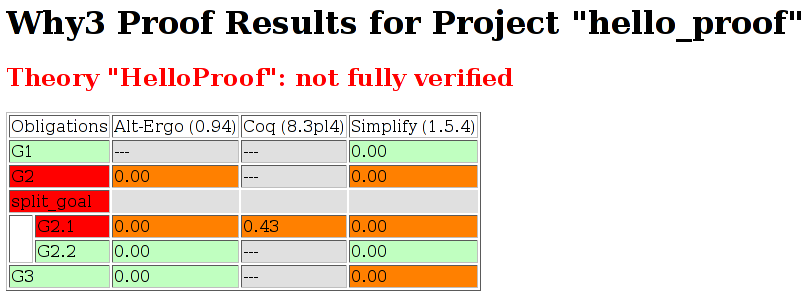
\includegraphics[width=0.9\textwidth]{hello_proof.png}}
  \end{center}
  \caption{HTML table produced for the HelloProof example}
\label{fig:html}
\end{figure}

The style 'table' outputs the contents of the session as a table,
similar to the LaTeX output above. Figure~\ref{fig:html} is the HTML table
produced for the 'HelloProof' example, as typically shown in a Web
browser.

The style ''simpletree' displays the contents of the session under the form of tree, similar to the tree view in the IDE. It uses only basic HTMl tags such as \verb|<ul>| and \verb|<li>|.

The style 'jstree' displays a dynamic tree view of the session, where
you can click on various parts to expand or shrink some part of the
tree. Clicking on a edited proof script also shows the contents of
this script. Technically, it use the 'jstree' plugin of the javascript
library 'jquery'.

Specific options for this command are as follows.
\begin{description}
\item[\texttt{-{}-style <s>}] sets the style to use, among
  \texttt{simpletree}, \texttt{jstree} and \texttt{table}, defaults to
  \texttt{table}.

\item[\texttt{-o}] the directory to output the produces files ('-' for
  stdout). The default is to output in the same directory as the session
  itself.

\item[\texttt{-{}-context}] adds context around the generated code in
  order to allow direct visualisation (header, css, ...). It also adds
  in the output directory all the needed external files. It can't be set with
  stdout output.

\item[\texttt{-{}-add\_pp <suffix> <cmd> <out\_suffix>}] adds for the
  given prefix the given pretty-printer, the new file as the given
  out\_suffix. cmd must contain '\%i' which will be replaced by the
  input file and '\%o' which will be replaced by the output file.

\item[\texttt{-{}-coqdoc}] use the \verb|coqdoc| command to display Coq proof
  scripts. This is equivalent to \texttt{-{}-add\_pp .v "coqdoc
    -{}-no-index -{}-html -o \%o \%i" .html}

\end{description}

\subsection{Commands modifying the proof attempts}

The subcommands \texttt{mod}, \texttt{copy}, \texttt{copy-archive},
and \texttt{rm} share the same set of options for selecting the proof
attempts to work on:
\begin{itemize}
\item Option \verb|--filter-prover| selects only the proof attempt with
  the given prover. This option can be specified multiple times to
  allow to select all the proofs that corresponds to one of the given
  provers. If this option is not specified, the proof are simply not
  filtered by there corresponding prover.
\item Option \verb|--filter-verified yes| restricts the selection to
  the proofs that are valid and not obsolete. On contrary the option
  \verb|--filter-verified no| select the ones that are not verified.
  \verb|--filter-verified all|, the default, does not select on this property.
\item Option \verb|--filter-verified-goal yes| restricts the selection
  to the proofs of verified goals (that does not mean that the proof is
  verified). Same for the other cases \verb|no| and \verb|all|.
\item Option \verb|--filter-archived yes| restricts the selection
  to the proofs that are archived.
  Same for the other cases \verb|no|
  and \verb|all| except the default is \verb|no|.
\end{itemize}

\noindent
The subcommand \texttt{mod}, \texttt{copy} and \texttt{copy-archive}
share the same set of option to specify the modification. The
subcommand \texttt{mod} modify directly the proof attempt,
\texttt{copy} copy the proof attempt before doing the modification,
\texttt{copy-archive} mark the original proof attempt as
archived.
The options are:
\begin{itemize}
\item Option \verb|--set-obsolete| marks the selected proofs as
  obsolete.
\item Option \verb|--set-archived| marks the selected proofs as archived.
\item Option \verb|--unset-archived| removes the archived attribute
  from the selected proofs.
\item Option \verb|--to-prover| modify the prover, for example
  \texttt{-{}-to-prover Alt-Ergo,0.94}. A conflict arises if a proof
  with this prover already exists. In this case you can choose between four
  behaviors:
\begin{itemize}
\item replace the proof (\verb|-f|, \verb|--force|);
\item do not replace the proof (\verb|-n|, \verb|--never|);
\item replace the proof unless it is verified (valid and not
  obsolete) (\verb|-c|, \verb|--conservative|); this is the default;
\item ask the user each time the case arises (\verb|-i|, \verb|--interactive|).
\end{itemize}
\end{itemize}


The subcommand \texttt{rm} removes the selected proof
attempts. The options \verb|-i, --interactive|, \verb|-f, --force| and
\verb|-c, --conservative| can also be used to respectively ask before
each suppression, suppress all the selected proof (default) and remove
only the proof that are not verified. The macro option \verb|--clean|
corresponds to \verb|--filter-verified-goal --conservative| and
removes the proof attempts that are not verified but which correspond
to verified goals.

The subcommands of this section don't accept by default to modify an
obsolete session (as defined in \ref{sec:idref:session}). You need to
add the option \verb|-F| to force this behavior.


% pour l'instant on ne documente pas parce que commenté dans le code
% \todo{A adapter en fonction de la decision sur l'upgrade de prover}

% If you just want to update one session with updated provers you can
% use \verb|--convert-unknown| instead of the option \verb|--to-prover|.
% \begin{verbatim}
% why3session copy  --convert-unknown
% \end{verbatim}
% For each proof attempt associated to an unknown prover (a prover not in
% \verb|.why3.conf|) and not archived, it will try to find a known prover
% with the same name. If it finds one, the proof attempt is copied to this
% prover and the old proof is set to archived. The corresponding edited
% files, if any, are copied and regenerated for the new prover An archived
% proof is not replayed by why3replayer.



\section{The \texttt{why3doc} tool}
\label{sec:why3doc}

This tool can produce HTML pages from \why source code. A source file
is scanned, \why code for theories or modules is output in
preformatted HTML code. Comments are interpreted in three different ways.
\begin{itemize}
\item Comments starting with at least three stars are completed
  ignored.
\item Comments starting with two stars are interpreted as textual
  documentation. Special constructs are interpreted as described
  below.
\item Comments starting with one star only are interpreted as code
  comments, and are typeset as the code
\end{itemize}

Additionally, all the \why identifiers are typeset with links so that
one can navigate through the HTML documentation, going from some
identifier use to its definition.

\paragraph{Options}

\begin{itemize}
\item Option \texttt{-o \textsl{<dir>}} defines the directory where to
  output the HTML files.
\item Option \verb|--output| is the same as \verb|-o|.
\item Option \verb|--index| (resp. \verb|--no-index|) to include
  (resp. exclude) the generation of an index file \texttt{index.html}.
  The default behavior is to generate an index if more than one file
  is passed on the command line.
\item Option \verb|--title|~\textsl{s} sets title \textsl{s} for the
  index page.
\item Option \verb|--stdlib-url|~\textsl{url} sets a URL for files
  found in load path, so that links to definitions can be added.
\end{itemize}

\paragraph{Typesetting textual comments}

Some constructs are interpreted:
\begin{itemize}
\item \texttt{\{\textsl{c text}\}} interprets character \textsl{c} as
  some typesetting command, detailed below
\item \texttt{[\textsl{code}]} is a code escape: the text
  \textsl{code} is typeset as \why code.
\end{itemize}

The typesetting commands are
\begin{description}
\item[1-6] a heading of level 1 to 6 respectively
\item[h] raw HTML
\end{description}

The HTML rendering is controlled via a CSS file \verb|style.css|
generated in the same directory as output files. This CSS style can be
modified manually: regenerating the doc will not overwrite an existing
\verb|style.css| file.



%%% Local Variables:
%%% mode: latex
%%% TeX-PDF-mode: t
%%% TeX-master: "manual"
%%% End:
